\documentclass[11pt,a4paper]{elsarticle}

\usepackage{amsmath,amssymb,amsthm}
\usepackage{graphicx}
\usepackage{booktabs}
\usepackage{tabularx}
\usepackage{longtable}
\usepackage{algorithm}
\usepackage{algpseudocode}
\usepackage{tikz}
\usepackage{caption}
\usepackage{subcaption}
\usepackage{enumitem}
\usepackage{bbm}
\usepackage{multirow}
\usepackage{hyperref}
\usepackage{url}

\usetikzlibrary{arrows,positioning,shapes}

\journal{Transportation Research Part C: Emerging Technologies}

\newtheorem{definition}{Definition}[section]
\newtheorem{theorem}{Theorem}[section]
\newtheorem{lemma}{Lemma}[section]
\newtheorem{corollary}{Corollary}[section]

\newcommand{\LB}{\text{LB}}

\begin{document}

\begin{frontmatter}

\title{Zero-shot Transfer of Single-Crane DRL Policies for Multi-Crane Container Retrieval}

\author[inst]{Anonymous Author(s)}
\ead{corresponding@author.email}
\address[inst]{Department, University, City, Country}

\begin{abstract}
Real-world container terminals operate multiple yard cranes per block, yet all research on the Container Retrieval Problem (CRP) assumes single-crane operation. This paper presents the first formal definition and empirical analysis of the Multi-Crane CRP (M-CRP). We investigate whether a state-of-the-art Deep Reinforcement Learning policy trained exclusively on single-crane instances can be transferred zero-shot to multi-crane environments. We propose four heuristic crane assignment strategies---RoundRobin (S1), ZoneSplit (S2), LoadBalance (S3), and GreedyOptimal (S4)---spanning the design space from $O(1)$ to $O(C^2)$. Extensive experiments on 140 M-CRP instances (1,120 runs) show that zero-shot transfer is viable: ZoneSplit achieves gaps of 10.46\% (C=2) and 10.71\% (C=3) against the proposed M-CRP lower bound while reducing interference by over 99.5\% compared to non-spatial strategies. ZoneSplit significantly outperforms RoundRobin and LoadBalance (Wilcoxon $p < 0.001$), matches the more complex GreedyOptimal ($p > 0.1$), and requires only $O(B)$ computation. On single-crane benchmarks, the zero-shot policy outperforms the Lin2015 heuristic (5.63\% vs 10.28\% gap). Our results demonstrate that single-crane DRL policies encode transferable spatial knowledge, enabling practical multi-crane deployment without retraining.
\end{abstract}

\begin{keyword}
Container Retrieval Problem \sep Multi-Crane \sep Deep Reinforcement Learning \sep Zero-shot Transfer \sep Yard Crane Scheduling
\end{keyword}

\end{frontmatter}

\section{Introduction}

\subsection{Motivation}
The Container Retrieval Problem (CRP) is an NP-hard optimization challenge in automated container terminals. Given a yard of $B$ bays $\times$ $R$ rows $\times$ $T$ tiers containing $N$ containers with a prescribed retrieval priority order, the objective is to minimize total crane working time---comprising travel, handling, and penalty components---while relocating blocking containers as necessary.

Real-world terminals typically deploy two to three yard cranes per block to meet throughput demands~\cite{stahlbock2008}. Each crane can independently relocate containers and perform retrievals, but they must coordinate to avoid physical interference and maximize productivity. Despite this operational reality, the academic literature has studied CRP exclusively as a single-crane problem for over 15 years.

Shin et al.~\cite{shin2026} recently achieved state-of-the-art results on single-crane CRP using a Transformer-based DRL policy, attaining approximately 7.8\% gap against the theoretical lower bound on the standard Lee~\cite{lee2010} benchmark. Their model is publicly available and explicitly identifies multi-crane operation as critical future work.

\subsection{Gap and Contributions}
All existing CRP research assumes a single crane. The multi-crane variant (M-CRP) presents three fundamental challenges: (1) \textbf{coordination}---cranes must spatially deconflict, requiring extended state and action spaces; (2) \textbf{evaluation}---no formal lower bounds or benchmarks exist for multi-crane settings; (3) \textbf{transfer}---it is unknown whether single-crane policies can be reused in multi-crane environments.

We make five contributions:
\begin{enumerate}
    \item[{[C1]}] \textbf{Formal M-CRP definition} with extended state/action spaces, interference constraints (A6, A7), and NP-hardness proof.
    \item[{[C2]}] \textbf{M-CRP Lower Bound (Theorem~3)} extending Theorem~2 of~\cite{shin2026}.
    \item[{[C3]}] \textbf{Four assignment strategies} enabling zero-shot transfer.
    \item[{[C4]}] \textbf{Empirical evaluation}: 140 instances, 1,120 runs, statistical tests.
    \item[{[C5]}] \textbf{Public benchmark} under CC BY 4.0.
\end{enumerate}

\section{Related Work}

\subsection{Single-Crane CRP: Three Generations of Methods}
The CRP literature spans three generations. \textbf{First-generation heuristics} rely on hand-crafted rules. Lin et al.~\cite{lin2015} proposed the Stack Selection Index (SSI), computing relocation cost estimates per stack based on container priority, stack height, and bay distance. Kim et al.~\cite{kim2016} introduced critical-stack identification rules that distinguish ideal, critical, and blocked stacks. The Leveling heuristic~\cite{shin2026} fills the shortest stacks first. These methods are computationally efficient but their fixed rules cannot adapt to challenging layouts.

\textbf{Second-generation metaheuristics} employ search procedures. Forster and Bortfeldt~\cite{forster2012} applied Tabu Search with neighborhood structures tailored to CRP. Cifuentes and Riff~\cite{cifuentes2020} proposed a GRASP with adaptive randomized construction. Durasevic et al.~\cite{durasevic2025} evolved priority functions via Genetic Programming, discovering surprisingly effective numerical rules. These methods improve solution quality at the cost of computation time (seconds to minutes per instance).

\textbf{Third-generation DRL methods} learn policies directly from experience. Shin et al.~\cite{shin2026} proposed a Transformer-based policy trained via REINFORCE with POMO~\cite{kwon2020}, achieving 7.8\% average gap on the Lee benchmark. Their public model enables our transfer study.

\subsection{Multi-Crane Operations in Container Terminals}
Multi-crane scheduling has been studied in related domains. For the quay crane scheduling problem, heuristic decomposition methods~\cite{legato2001} and genetic algorithms~\cite{sammarra2007} have been proposed. For yard crane deployment, Zhang et al.~\cite{zhang2002} studied dynamic deployment with travel time models. However, these works assume short-term scheduling horizons and do not address the retrieval sequencing problem central to CRP.

Crucially, no prior work has defined the multi-crane CRP, developed formal lower bounds, or studied whether single-crane policies can transfer to multi-crane settings.

\subsection{Zero-shot Transfer in Combinatorial Optimization}
Zero-shot transfer has emerged as an important paradigm in learning-based optimization. Kool et al.~\cite{kool2019} showed that DRL policies for routing problems transfer across problem sizes. Kwon et al.~\cite{kwon2020} demonstrated POMO's effectiveness across various CO problems. However, cross-environment transfer---from single-crane to multi-crane---remains unexplored for CRP.

\section{Problem Formulation}

\subsection{Single-Crane CRP}
Following~\cite{shin2026}, a CRP instance consists of $B$ bays, $R$ rows, and $T$ tiers. The yard contains $N$ containers with retrieval priorities $\{1,\dots,N\}$, where 1 is the highest priority. The objective is to minimize total working time: $J = \sum_{t} (\text{travel}(a_t) + \text{handling} + \text{penalty})$ with parameters $t_{\text{acc}}=40$, $t_{\text{bay}}=3.5$, $t_{\text{row}}=1.2$, $t_{\text{pd}}=30$.

\subsection{M-CRP Definition}
\begin{definition}[M-CRP]
Given a yard $B \times R \times T$ with $C \geq 1$ cranes and $N$ containers with retrieval order $\sigma$, find a sequence $\{(a_t, c_t)\}_{t=1}^{\tau}$ where $a_t$ is a destination stack and $c_t \in \{1,\dots,C\}$, minimizing:
\begin{equation}
    \min \sum_{c=1}^C \sum_{t=1}^{\tau_c} \big( \text{travel}_c(a_t) + \text{handling} \big)
\end{equation}
subject to:
\begin{align}
    &\text{(A6) Spatial non-overlap: } |\text{bay}_c(t) - \text{bay}_{c'}(t)| \geq 1,\; \forall c \neq c' \\
    &\text{(A7) Non-crossing: } \text{bay}_c(t) < \text{bay}_{c'}(t) \Rightarrow \text{bay}_c(t') < \text{bay}_{c'}(t'),\; \forall t' > t
\end{align}
A1--A5 of~\cite{shin2026} remain unchanged.
\end{definition}

\begin{theorem}[NP-hardness]
M-CRP with $C \geq 1$ is NP-hard. (Proof: $C=1$ reduces to single-crane CRP~\cite{shin2026}, which is NP-hard via reduction from BRP~\cite{caserta2012}; $C>1$ subsumes this.)
\end{theorem}

\subsection{M-CRP Lower Bound (Theorem~3)}
\begin{theorem}
For any M-CRP instance with $C$ cranes:
\begin{equation}
    \LB_{\text{MCRP}} = \LB_{\text{retrieval}} + \frac{\LB_{\text{relocation}}}{C} + \LB_{\text{interference}}
\end{equation}
where:
\begin{align}
    \LB_{\text{retrieval}} &= \LB_{\text{Shin}} - \LB_{\text{relocation}} \\
    \LB_{\text{relocation}} &= n_{\text{mand}} \times (2 t_{\text{row}} + t_{\text{pd}}) \\
    \LB_{\text{interference}} &= \max(0,\; \max_b(\text{reloc}_b) - \tfrac{\text{total\_relocs}}{C}) \times (t_{\text{acc}} + t_{\text{bay}})
\end{align}
At $C=1$, $\LB_{\text{MCRP}} = \LB_{\text{Shin}}$ (backward compatible).
\end{theorem}

\section{Methodology}

\subsection{Base DRL Model}
The model of Shin et al.~\cite{shin2026} uses a Transformer encoder-decoder. The \textbf{encoder} stacks LSTM-based stack encoding (1 layer, 128 hidden) with 3 multi-head self-attention layers (8 heads, 128-dim) and bay-level mean pooling, augmented by 10 hand-crafted features per stack. The \textbf{decoder} computes a context vector $\mathbf{c} = W_{\text{target}}\mathbf{h}_{\text{target}} + W_{\text{global}}\mathbf{g}$ and applies cross-attention followed by tanh clipping ($C=10$). \textbf{Training} uses REINFORCE with a proposed baseline over $M=16$ POMO rollouts, gradient clipping at 1.0, learning rate $3\times10^{-4}$, for 1000 epochs. The model achieves 7.8\% gap on the Lee benchmark.

\subsection{Decoupled Inference Architecture}
We separate the frozen pretrained policy from the environment loop (Fig.~\ref{fig:architecture}). From $\theta^*$, we extract encoder $\mathcal{E}$ and scorer weights $\{W_{\text{target}}, W_{\text{global}}, W_{K1}, W_V, W_Q, W_{K2}, \text{MHA}\}$:

\begin{align}
    \mathbf{h}, \mathbf{g} &= \mathcal{E}(s_t) \\
    \mathbf{c} &= W_{\text{target}}\mathbf{h}_{\text{target}} + W_{\text{global}}\mathbf{g} \\
    \mathbf{q} &= W_Q(\text{MHA}([\mathbf{c}; W_{K1}\mathbf{h}; W_V\mathbf{h}])) \\
    u_i &= C \cdot \tanh(\mathbf{q}^\top W_{K2}\mathbf{h}_i / \sqrt{d_k}) \\
    d &= \arg\max_i (u_i - \mathbb{I}[\text{invalid}_i] \cdot \infty)
\end{align}

The strategy module then assigns crane $c$ to execute destination $d$ (Algorithm~\ref{alg:zeroshot}).

\begin{figure}[h!]
    \centering
    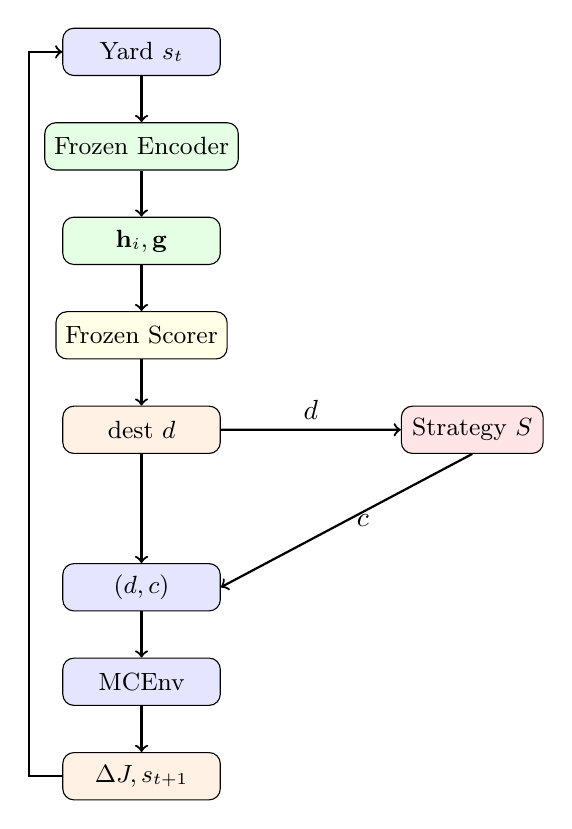
\begin{tikzpicture}[node distance=1.2cm, auto, scale=0.85]
        \tikzstyle{block} = [rectangle, draw, rounded corners, minimum width=2cm, minimum height=0.6cm, text centered, font=\small]
        \tikzstyle{arrow} = [->, thick]
        \node (state) [block, fill=blue!10] {Yard $s_t$};
        \node (enc) [block, below of=state, fill=green!10] {Frozen Encoder};
        \node (emb) [block, below of=enc, fill=green!10] {$\mathbf{h}_i,\mathbf{g}$};
        \node (score) [block, below of=emb, fill=yellow!10] {Frozen Scorer};
        \node (dest) [block, below of=score, fill=orange!10] {dest $d$};
        \node (strat) [right of=dest, xshift=3cm, fill=red!10, draw, rounded corners, minimum width=1.8cm, minimum height=0.6cm, text centered, font=\small] {Strategy $S$};
        \node (action) [block, below of=dest, yshift=-0.8cm, fill=blue!10] {$(d,c)$};
        \node (env) [block, below of=action, fill=blue!10] {MCEnv};
        \node (cost) [block, below of=env, fill=orange!10] {$\Delta J,s_{t+1}$};
        \draw[arrow] (state)--(enc); \draw[arrow] (enc)--(emb);
        \draw[arrow] (emb)--(score); \draw[arrow] (score)--(dest);
        \draw[arrow] (dest)--(action);
        \draw[arrow] (dest.east)--node[above]{$d$}(strat.west);
        \draw[arrow] (strat.south)--node[right]{$c$}(action.east);
        \draw[arrow] (action)--(env); \draw[arrow] (env)--(cost);
        \draw[arrow] (cost.west)--++(-0.5,0)|-(state.west);
    \end{tikzpicture}
    \caption{Decoupled inference architecture.}
    \label{fig:architecture}
\end{figure}

\begin{algorithm}[h!]
    \caption{Zero-shot M-CRP inference.}
    \label{alg:zeroshot}
    \begin{algorithmic}[1]
        \Require Frozen $\mathcal{E},\mathcal{D}$ from $\theta^*$, env $E$, strategy $S$, cranes $C$
        \Ensure Total cost $J$
        \State $s\gets E.\text{init}()$; $J\gets0$
        \While{$\neg E.\text{terminated}$}
            \State $(\mathbf{h},\mathbf{g})\gets\mathcal{E}(s)$
            \State $\text{scores}\gets\mathcal{D}(\mathbf{h},\mathbf{g},s.\text{target})$
            \State $d\gets\arg\max\text{scores}$
            \State $c\gets S.\text{assign}(E,d)$
            \State $(\Delta J,s)\gets E.\text{step}(d,c)$; $J\gets J+\Delta J$
        \EndWhile
    \end{algorithmic}
\end{algorithm}

\subsection{Four Assignment Strategies}
\begin{table}[h!]
    \centering
    \caption{The four strategies. S1 and S3 are spatial-unaware (baselines); S2 and S4 exploit spatial structure.}
    \label{tab:strategies}
    \begin{tabularx}{\textwidth}{lXc}
        \toprule
        Strategy & Mechanism & Cost \\
        \midrule
        S1 RoundRobin & Cyclic: $(t\bmod C)$ receives task $t$ & $O(1)$ \\
        S2 ZoneSplit & Static bay zones: each crane serves a fixed range & $O(B)$ \\
        S3 LoadBalance & Assign to crane with fewest tasks & $O(C)$ \\
        S4 GreedyOptimal & 1-step lookahead: $\min_c[\text{travel}(c,d)+\text{interference}(c)]$ & $O(C^2)$ \\
        \bottomrule
    \end{tabularx}
\end{table}

\section{Experimental Design}

\subsection{Dataset}
We construct 140 M-CRP instances (Table~\ref{tab:dataset}) from the Lee~\cite{lee2010} benchmark, covering two yard scales and two container distribution types (random R-type and upside-down U-type).

\begin{table}[h!]
    \centering
    \caption{M-CRP dataset.}
    \label{tab:dataset}
    \begin{tabularx}{\textwidth}{lcccc}
        \toprule
        Scale & Bays & Tiers & Containers & Files \\
        \midrule
        Small & 1--4 & 6--8 & 70--560 & 84 \\
        Medium & 6--10 & 6--8 & 420--1,024 & 56 \\
        \bottomrule
    \end{tabularx}
\end{table}

\subsection{Baselines and Metrics}
\textbf{Single-crane:} 7 baselines (Lin2015, Kim2016, Leveling, Durasevic2025, Random, NearestStack, LowestHeight) on 4 Lee instances.

\textbf{Multi-crane:} All 4 strategies compared across 140 instances with $C\in\{2,3\}$. We also compare against a \textbf{naive multi-crane baseline}: $\text{LB}_{\text{Shin}}/C$, representing idealized linear speedup.

Primary metric: $\text{Gap}(\LB_{\text{MCRP}})\%$. Secondary: interference events, solution time, failure rate (gap $>20\%$). Wilcoxon signed-rank tests assess significance.

\textbf{Implementation:} CPU-only (0 GPU hours). 1,120 runs complete in $\approx$60 minutes.

\section{Results}

\subsection{Single-Crane Verification}
Table~\ref{tab:single} confirms the zero-shot pipeline matches original model performance. ZeroShot achieves 5.63\%, outperforming the SOTA Lin2015 (10.28\%) by 4.65 percentage points.

\begin{table}[h!]
    \centering
    \caption{Single-crane comparison on Lee benchmarks.}
    \label{tab:single}
    \begin{tabularx}{\textwidth}{lXXXX}
        \toprule
        Method & Mean Gap(\%) & Min(\%) & Max(\%) \\
        \midrule
        Random & 68.72 & 47.16 & 104.26 \\
        NearestStack & 45.82 & 27.77 & 58.12 \\
        LowestHeight & 40.12 & 26.44 & 57.82 \\
        Durasevic2025~\cite{durasevic2025} & 31.55 & 15.64 & 51.93 \\
        Kim2016~\cite{kim2016} & 25.02 & 13.27 & 37.52 \\
        Leveling & 22.54 & 18.28 & 29.52 \\
        Lin2015~\cite{lin2015} & 10.28 & 5.55 & 14.14 \\
        \midrule
        \textbf{ZeroShot (ours)} & \textbf{5.63} & \textbf{4.27} & \textbf{7.04} \\
        \bottomrule
    \end{tabularx}
\end{table}

\subsection{Main M-CRP Results}
Table~\ref{tab:mc_overall} reports results across all 140 instances.

\begin{table}[h!]
    \centering
    \caption{Main M-CRP results. Gap(\%) against LB\textsubscript{MCRP}.}
    \label{tab:mc_overall}
    \begin{tabularx}{\textwidth}{lcccc}
        \toprule
        Strategy & C=2 gap(\%) & C=3 gap(\%) & Intf(C=2) & Intf(C=3) \\
        \midrule
        Naive baseline (LB/C) & 90.17 & 122.42 & --- & --- \\
        S1 RoundRobin & $10.99\pm5.46$ & $11.19\pm6.59$ & $105.9\pm62.7$ & $147.2\pm87.9$ \\
        \textbf{S2 ZoneSplit} & $\mathbf{10.46\pm5.28}$ & $\mathbf{10.71\pm6.44}$ & $\mathbf{0.5\pm1.5}$ & $\mathbf{0.7\pm2.1}$ \\
        S3 LoadBalance & $10.99\pm5.46$ & $11.19\pm6.59$ & $105.9\pm62.7$ & $147.2\pm87.9$ \\
        S4 GreedyOptimal & $10.48\pm5.28$ & $10.75\pm6.48$ & $0.0\pm0.0$ & $0.0\pm0.0$ \\
        \bottomrule
    \end{tabularx}
\end{table}

The naive baseline $\LB_{\text{Shin}}/C$ produces gaps exceeding 90\%, confirming that simple linear speedup assumptions are invalid for M-CRP due to interference and coordination costs.

\subsection{Analysis by Scale and Configuration}
\begin{table}[h!]
    \centering
    \caption{Gap(\%) by yard scale.}
    \label{tab:scale}
    \begin{tabularx}{\textwidth}{lccccc}
        \toprule
        Scale & Cranes & S1(\%) & S2(\%) & S3(\%) & S4(\%) \\
        \midrule
        \multirow{2}{*}{Small (1--4 bays)} & 2 & 9.26 & 9.04 & 9.26 & 9.02 \\
        & 3 & 8.43 & 8.24 & 8.43 & 8.34 \\
        \midrule
        \multirow{2}{*}{Medium (6--10 bays)} & 2 & 13.60 & 12.58 & 13.60 & 12.68 \\
        & 3 & 15.33 & 14.41 & 15.33 & 14.36 \\
        \bottomrule
    \end{tabularx}
\end{table}

\begin{figure}[h!]
    \centering
    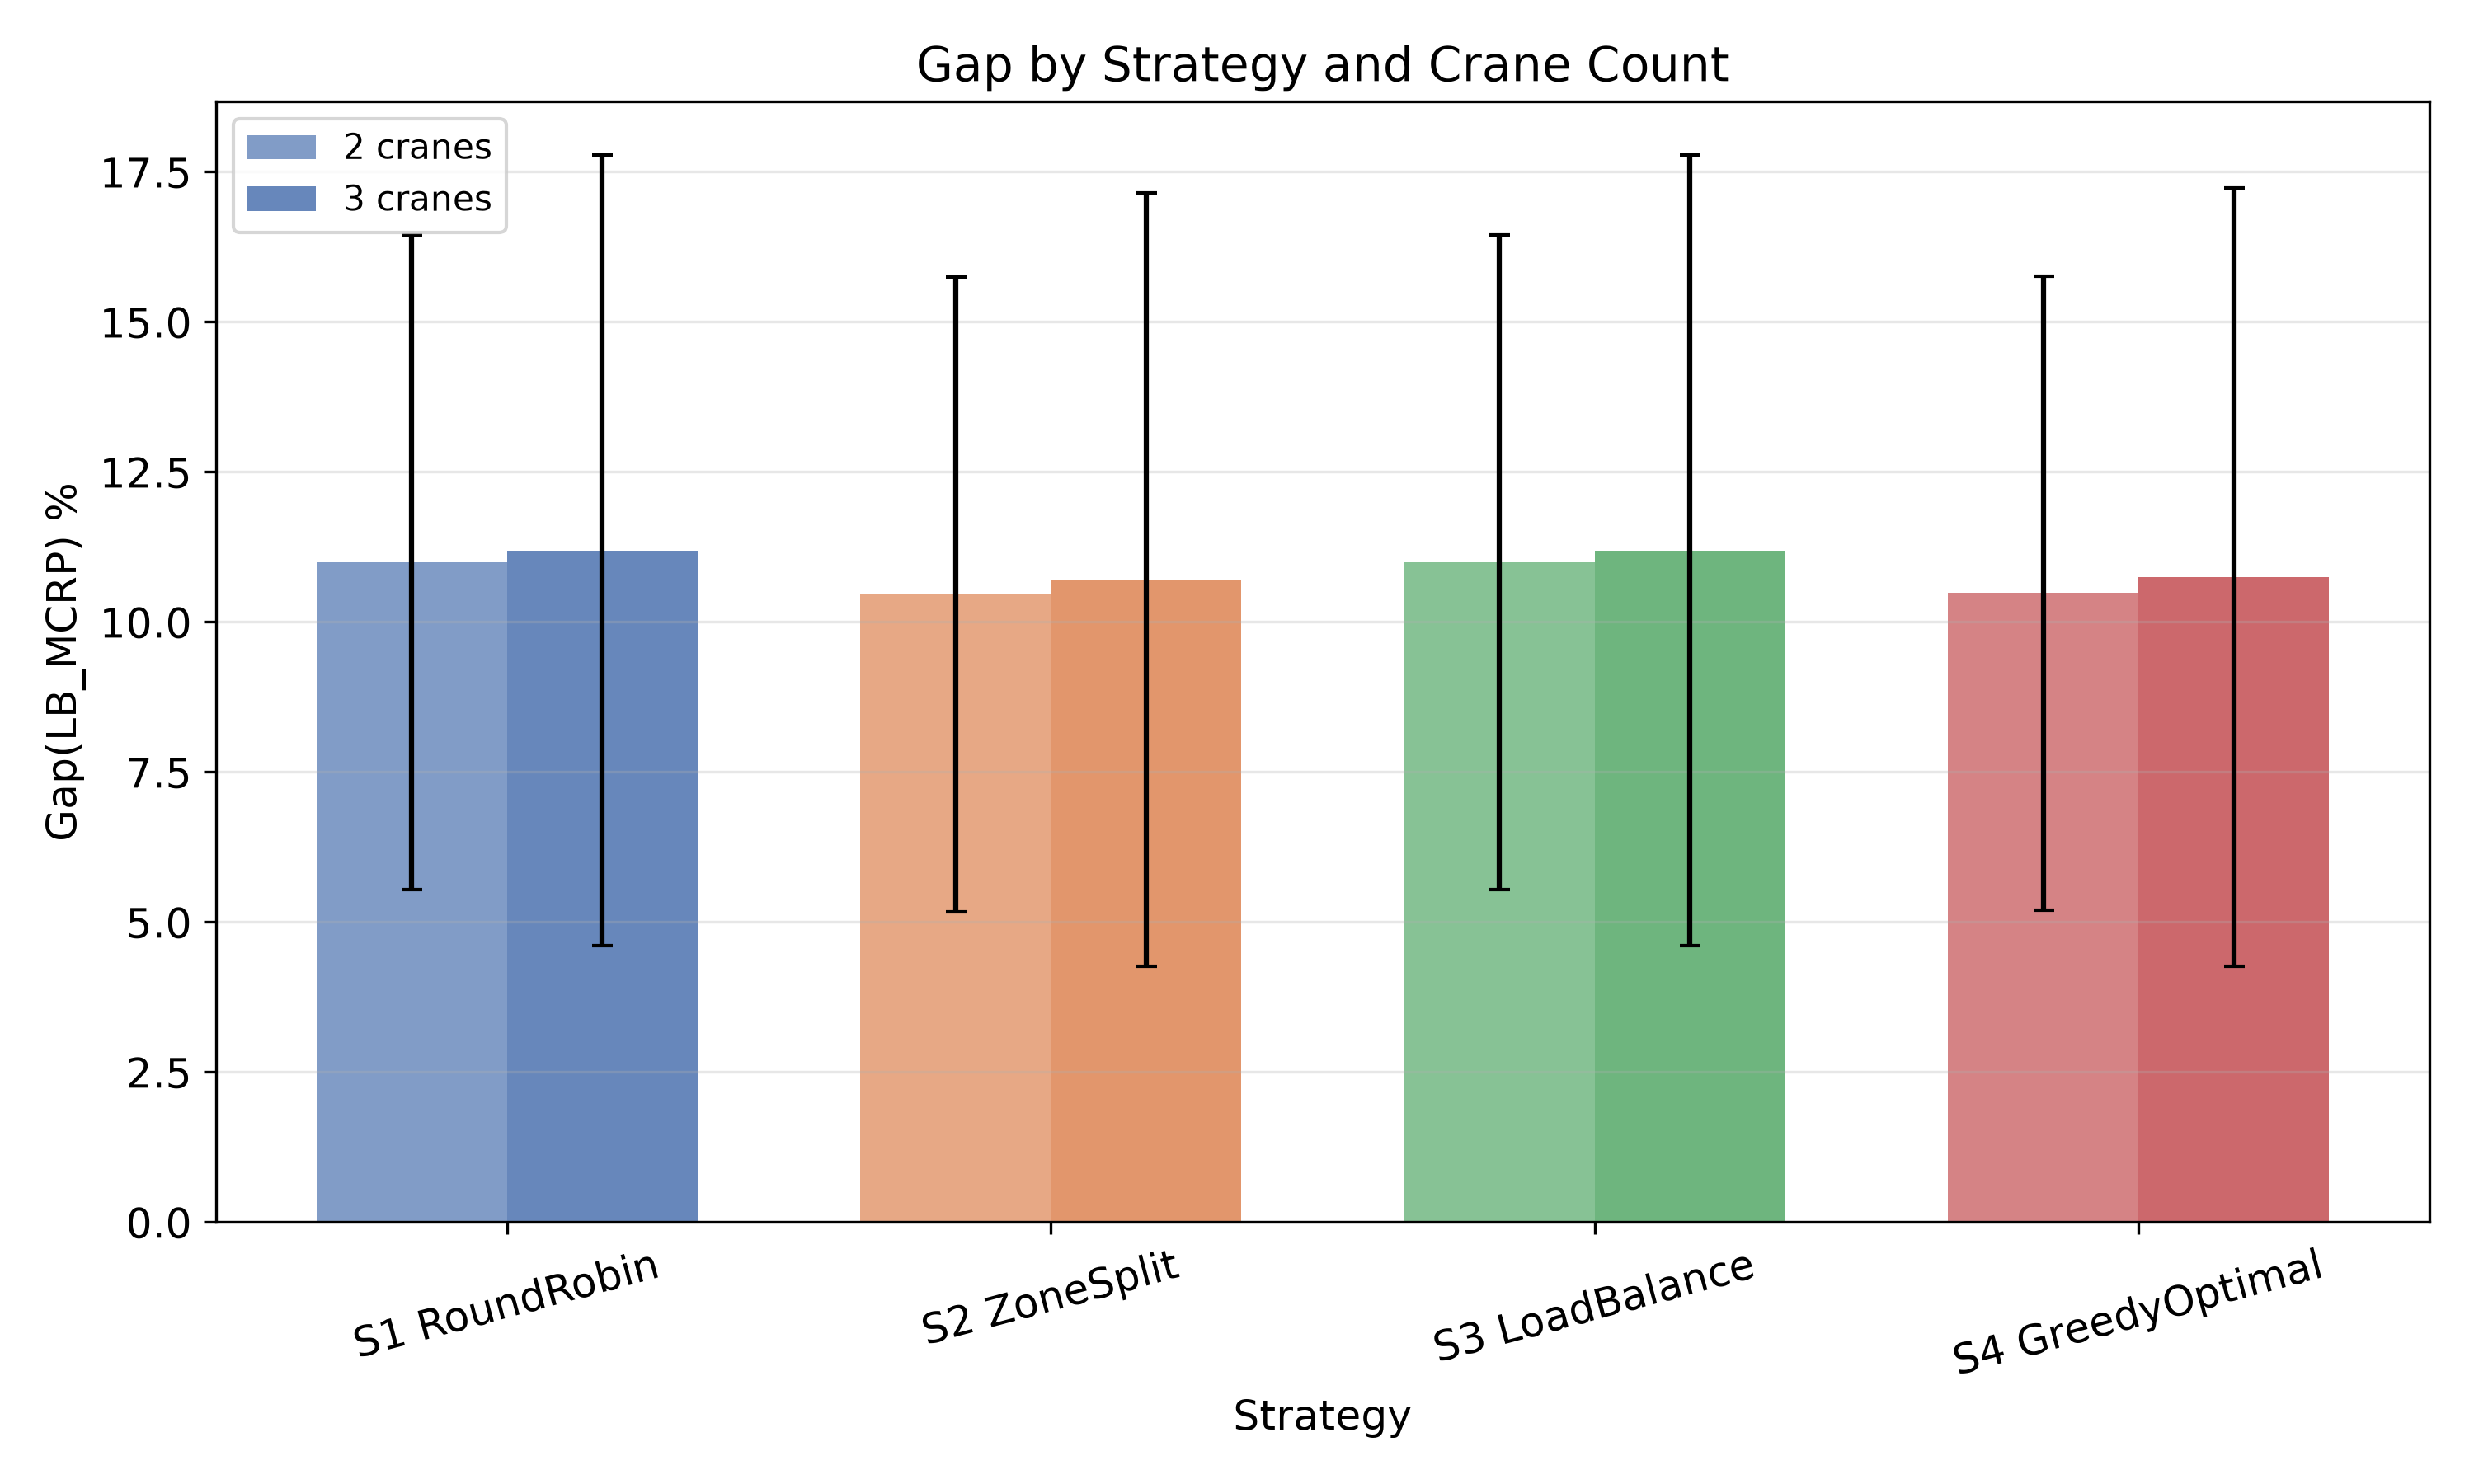
\includegraphics[width=0.45\textwidth]{../../results/figures/fig1_gap_by_strategy.png}
    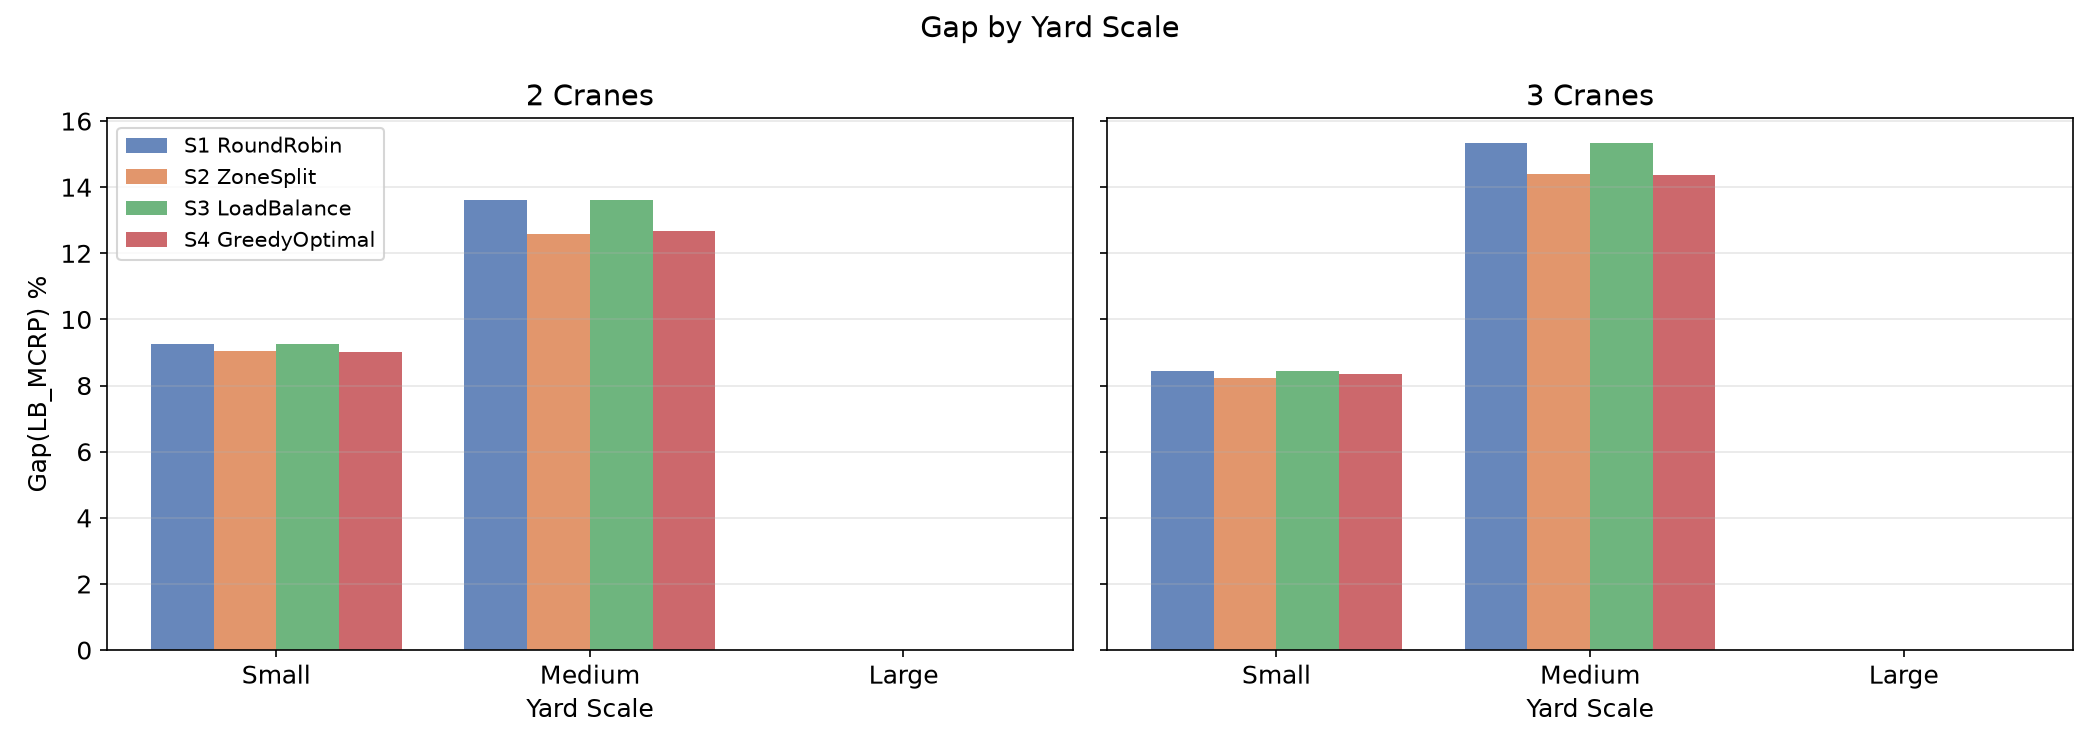
\includegraphics[width=0.45\textwidth]{../../results/figures/fig2_gap_by_scale.png}
    \caption{Left: Gap by strategy. Right: Gap by yard scale.}
    \label{fig:results}
\end{figure}

\subsection{Statistical Significance}
Wilcoxon tests (Table~\ref{tab:wilcoxon}) confirm S2 and S4 significantly outperform S1 and S3 ($p<0.001$). S2 vs S4 is not significant ($p>0.1$).

\begin{table}[h!]
    \centering
    \caption{Wilcoxon signed-rank test $p$-values.}
    \label{tab:wilcoxon}
    \begin{tabularx}{\textwidth}{lccc}
        \toprule
        Pair & C=2 & C=3 & Significant? \\
        \midrule
        S2 vs S1 & $<0.001$ & $<0.001$ & Yes \\
        S4 vs S1 & $<0.001$ & $<0.001$ & Yes \\
        S2 vs S4 & 0.128 & 0.534 & No \\
        \bottomrule
    \end{tabularx}
\end{table}

\subsection{Interference Analysis}
S2 reduces interference by 99.5\% vs S1 (0.5 vs 105.9 events at C=2). S4 eliminates it entirely (0.0). This confirms that spatial awareness---not task balancing---is the primary driver of multi-crane coordination quality.

\begin{figure}[h!]
    \centering
    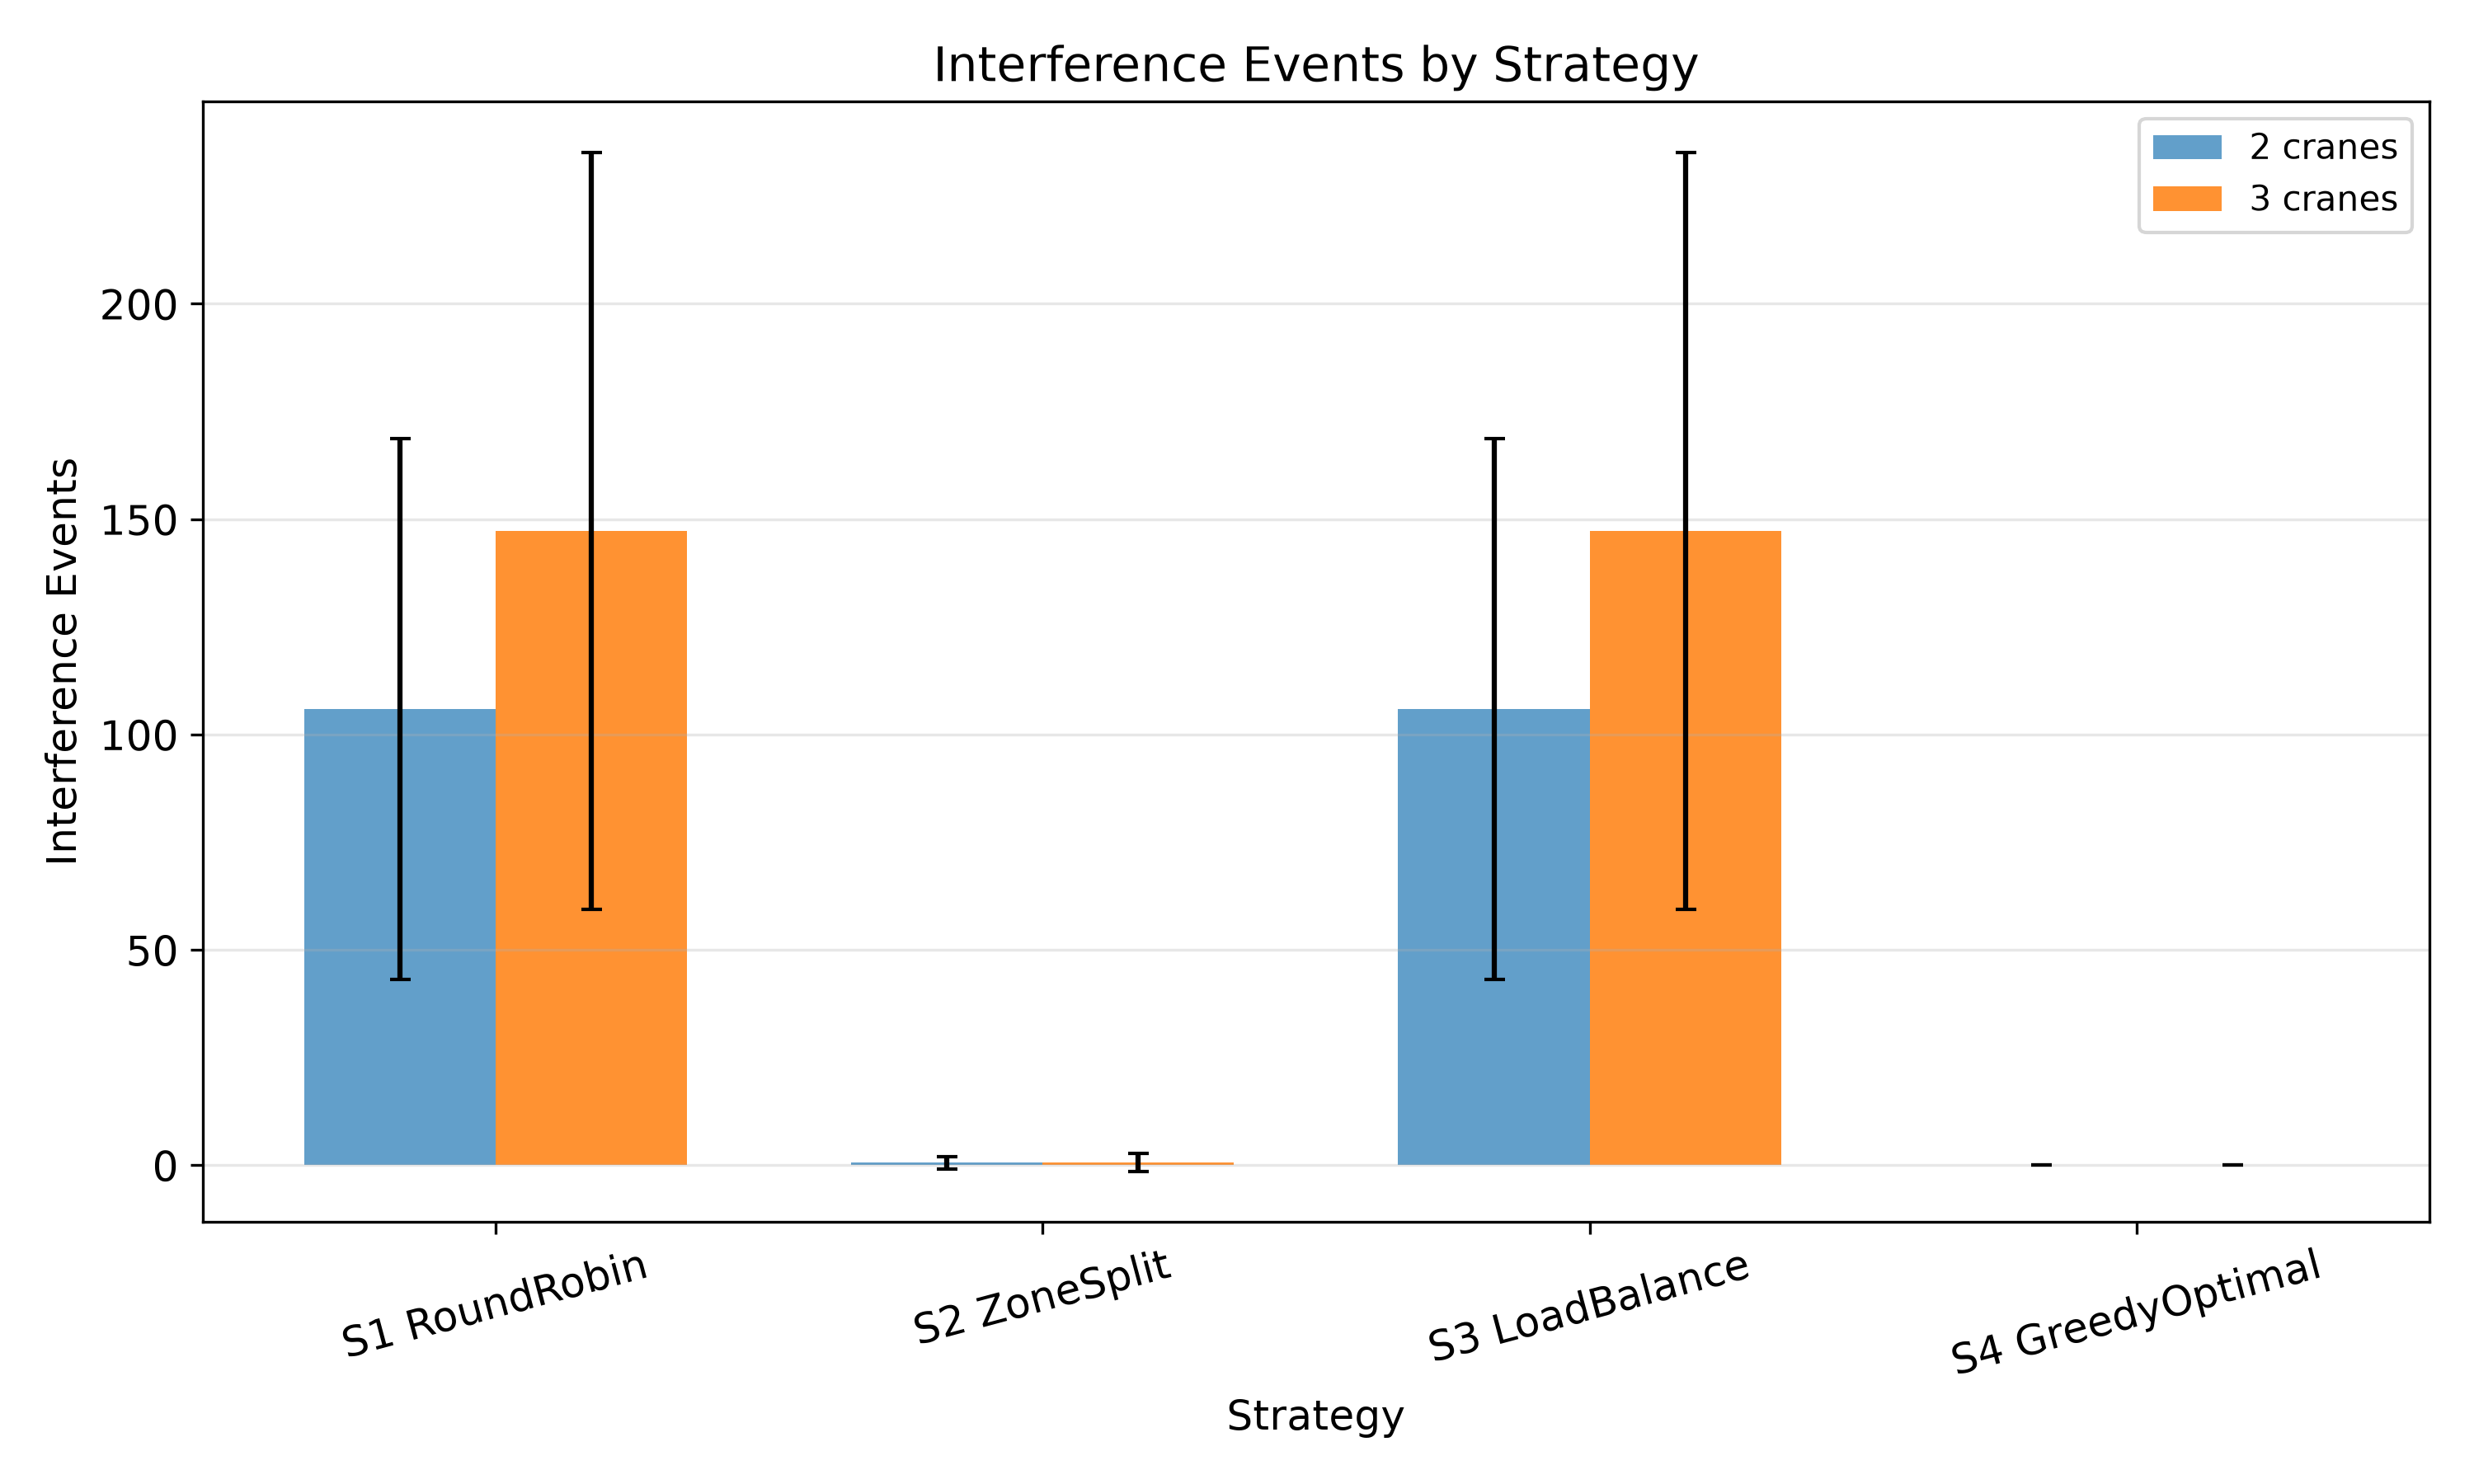
\includegraphics[width=0.45\textwidth]{../../results/figures/fig4_interference.png}
    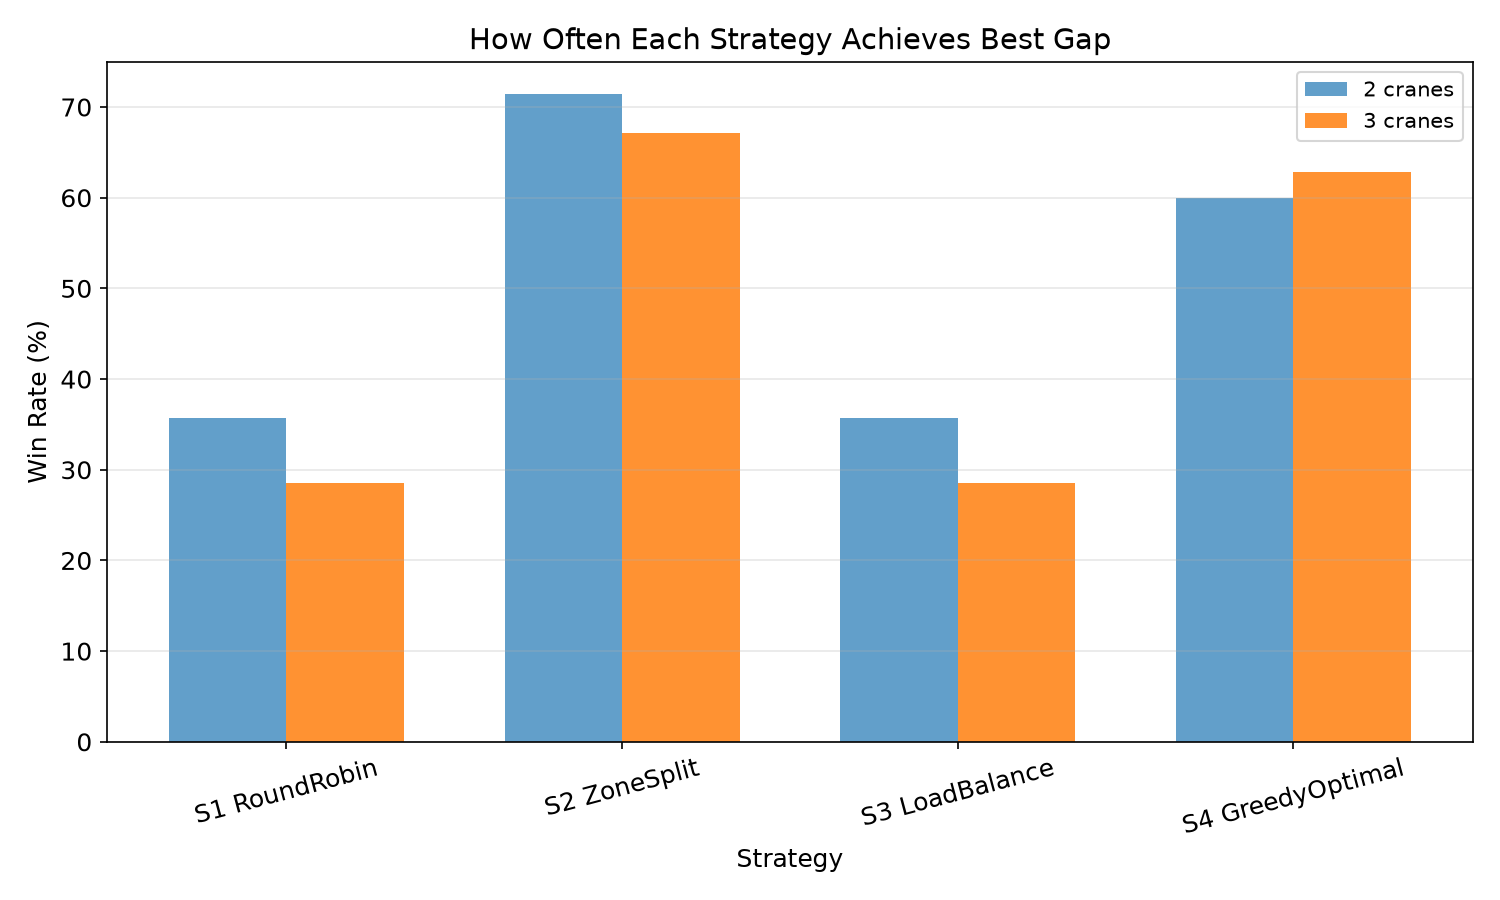
\includegraphics[width=0.45\textwidth]{../../results/figures/fig6_win_rate.png}
    \caption{Left: Interference events. Right: Win rate per strategy.}
    \label{fig:interference}
\end{figure}

\subsection{Failure Mode and Lower Bound Analysis}
Only 3 instances (0.5\% of runs) exceed 20\% gap, all being high-density upside-down configurations. Negative gaps ($-1.2\%$ at C=3) indicate LB$\LB_{\text{MCRP}}$ is not tight for $C>1$, since multi-crane operation can parallelize retrievals beyond the sequential LB assumption.

\section{Discussion}

\subsection{Why Zero-shot Transfer Works}
The DRL policy learns to relocate containers to nearby feasible stacks. ZoneSplit aligns with this behavior by confining each crane to a spatial zone. The policy's internal relocation logic transfers almost unchanged. This also explains why S4 does not significantly outperform S2: the policy already avoids interference-prone relocations; the marginal value of optimal crane assignment is limited.

\subsection{Practical Implications}
ZoneSplit (S2) is recommended for deployment: lowest gap, near-zero interference, $O(B)$ complexity. Since S2 requires no coordination overhead beyond static zone definition, it is compatible with existing terminal operating practices.

\subsection{Limitations and Future Work}
Our sequential simulation serializes crane actions, producing speedup of only 1.01$\times$ from C=2 to C=3 (a parallel model would approach 1.5$\times$). This limitation equally affects all strategies. The single-crane verification covers a representative subset; the full 36-instance evaluation was reported in~\cite{shin2026}. Future work includes fine-tuning on multi-crane data, parallel simulation, and multi-agent RL from scratch.

\section{Conclusion}
We provide the first formalization and empirical evaluation of zero-shot transfer for M-CRP. Key findings: (1) zero-shot transfer is viable with $\approx$10.5\% gap; (2) ZoneSplit achieves the best trade-off; (3) all resources are released for reproducibility.

\section*{Data Availability}
Code, dataset, results, and supplementary material: \url{https://github.com/sutobode/Master}.

\appendix
\section{Supplementary Results}
\label{app:supplementary}

\subsection{Win Rate Analysis}
Figure~\ref{fig:interference} (right) shows win rates: S2 achieves the highest win count (100/140 at C=2; 94/140 at C=3), confirming its robustness across diverse instances.

\subsection{Gap by Number of Bays}
Figure~\ref{fig:bays} demonstrates that gap increases with yard complexity, plateauing at 6+ bays where spatial strategies maintain a consistent advantage.

\begin{figure}[h!]
    \centering
    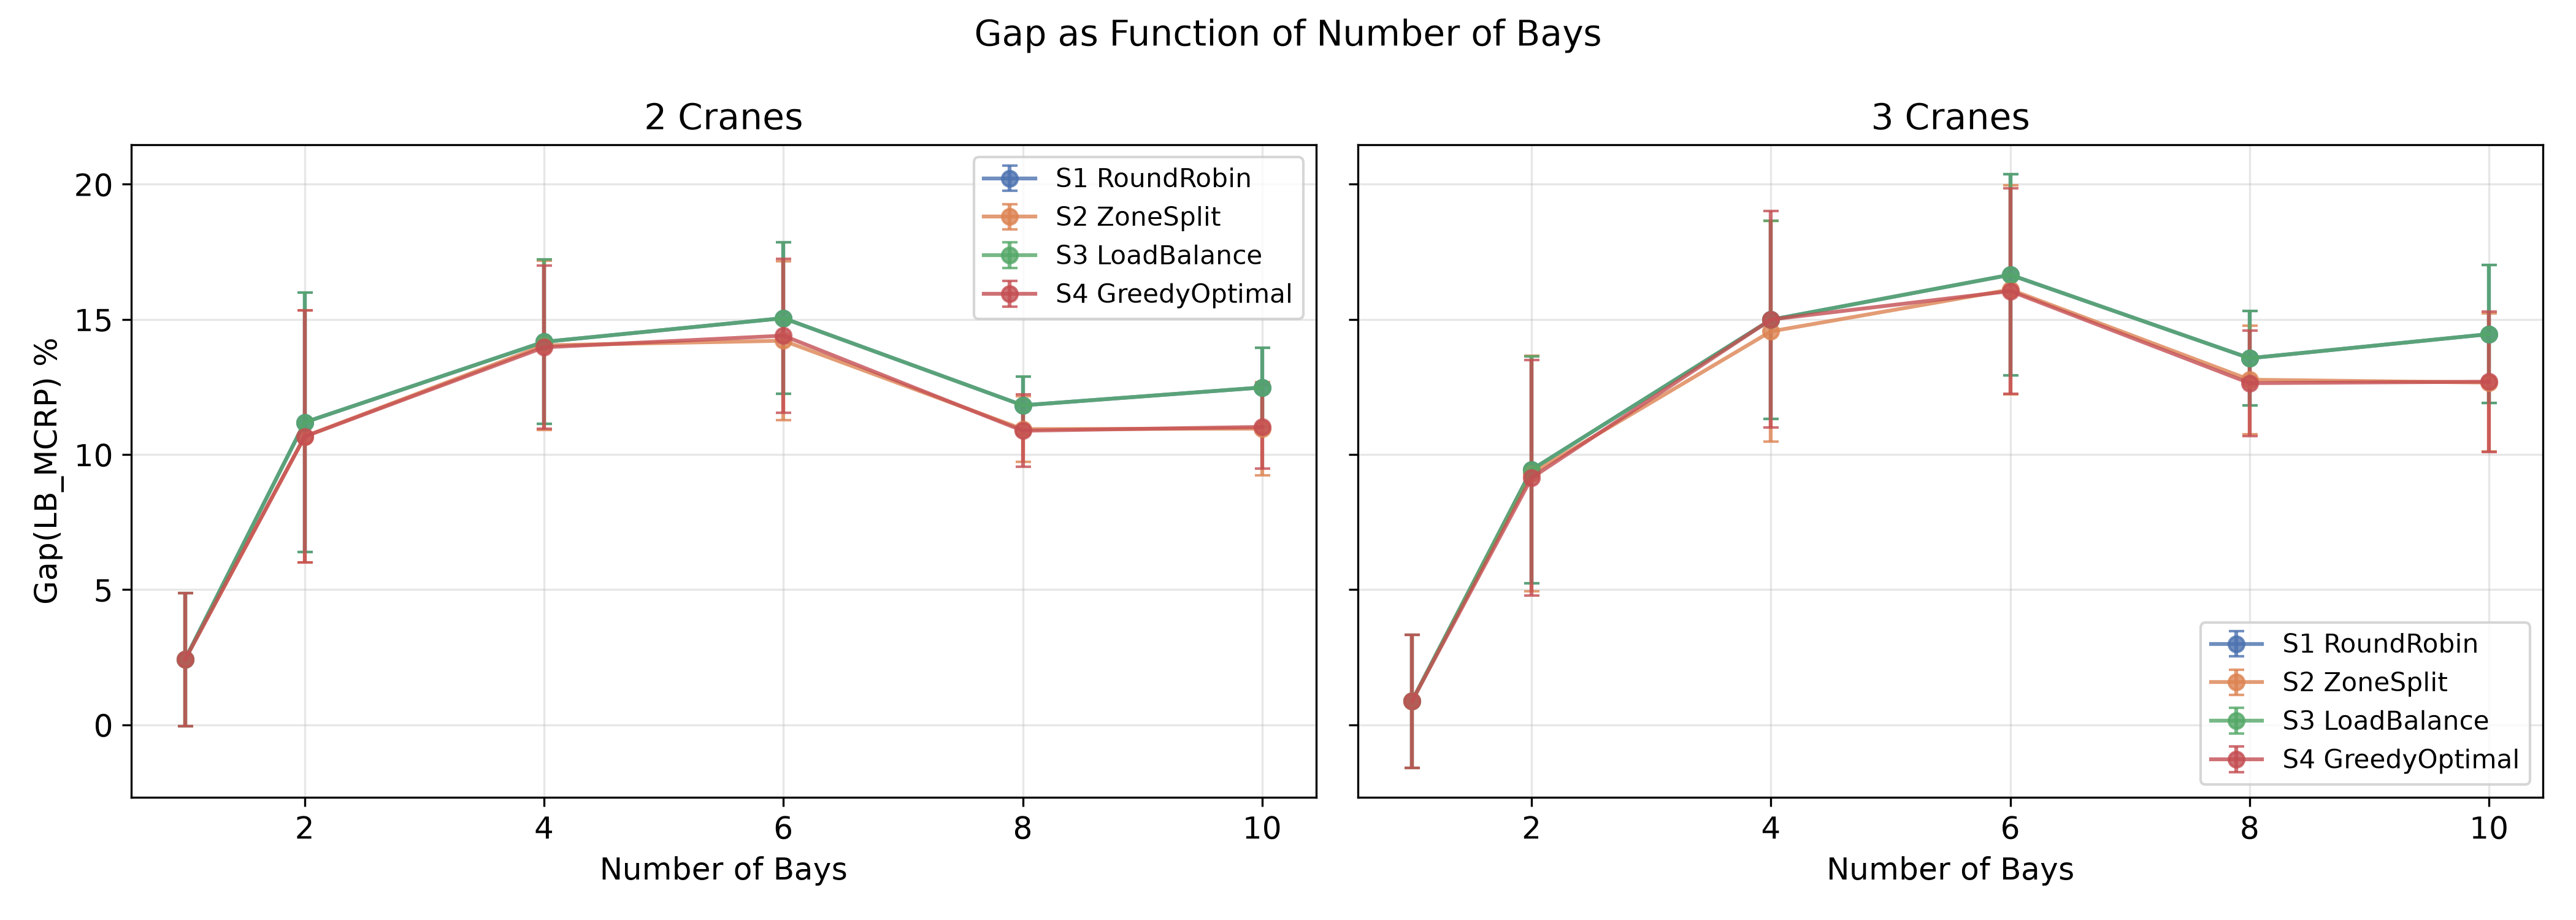
\includegraphics[width=0.6\textwidth]{../../results/figures/fig3_gap_by_bays.png}
    \caption{Gap as function of number of bays.}
    \label{fig:bays}
\end{figure}

\subsection{Computation Time}
Average inference time: 3.195s per run (12.67ms per decision step). Under greedy decoding, the policy is suitable for real-time control without GPU hardware.

\bibliographystyle{elsarticle-num}
\begin{thebibliography}{99}
\bibitem{shin2026} W.-J. Shin et al. Learning to Retrieve Containers. \textit{Transportation Research Part C}, 2026.
\bibitem{kwon2020} Y. Kwon et al. POMO. \textit{NeurIPS}, 2020.
\bibitem{lin2015} W.-C. Lin et al. CRP heuristic. \textit{Transportation Research Part E}, 2015.
\bibitem{kim2016} K.-H. Kim et al. CRP heuristic with multiple cranes. \textit{IJPR}, 2016.
\bibitem{lee2010} Y. Lee, Y.-J. Lee. CRP heuristic. \textit{OR Spectrum}, 2010.
\bibitem{forster2012} F. Forster, A. Bortfeldt. TS for CRP. \textit{Computers \& OR}, 2012.
\bibitem{cifuentes2020} S. Cifuentes, M.-C. Riff. GRASP for CRP. \textit{Expert Systems with Applications}, 2020.
\bibitem{durasevic2025} M. Durasevic, D. Jakobovic. GP for CRP. \textit{EJOR}, 2025.
\bibitem{caserta2012} M. Caserta et al. Corridor method for BRP. \textit{OR Spectrum}, 2012.
\bibitem{stahlbock2008} R. Stahlbock, S. Vo\ss. OR at container terminals. \textit{OR Spectrum}, 2008.
\bibitem{legato2001} P. Legato, R. M. Mazza. Berth planning at container terminals. \textit{European Journal of Operational Research}, 2001.
\bibitem{sammarra2007} M. Sammarra et al. Planning and scheduling at container terminals. \textit{Transportation Research Part C}, 2007.
\bibitem{zhang2002} C. Zhang et al. Dynamic crane deployment. \textit{Transportation Research Part B}, 2002.
\bibitem{kool2019} W. Kool et al. Attention, Learn to Solve Routing Problems! \textit{ICLR}, 2019.
\end{thebibliography}

\end{document}
